% Source: Lucas's set-equality template in IMG_9457.heic.
% Both branches are required proof obligations, rather than alternatives.
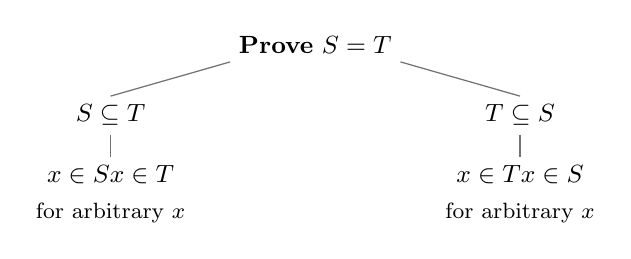
\begin{tikzpicture}[
  x=1cm,y=1cm,font=\small,
  every node/.style={inner sep=3pt,align=center},
  branch/.style={black!55,line width=0.45pt}
]
  \node (goal) at (0,0) {\textbf{Prove} \(S=T\)};
  \node (forward) at (-2.6,-0.9) {\(S\subseteq T\)};
  \node (reverse) at (2.6,-0.9) {\(T\subseteq S\)};
  \node (forward-elements) at (-2.6,-1.9)
    {\(x\in S\implies x\in T\)\\[2pt]
      {\footnotesize for arbitrary \(x\)}};
  \node (reverse-elements) at (2.6,-1.9)
    {\(x\in T\implies x\in S\)\\[2pt]
      {\footnotesize for arbitrary \(x\)}};
  \draw[branch] (goal.south west) -- (forward.north);
  \draw[branch] (goal.south east) -- (reverse.north);
  \draw[branch] (forward.south) -- (forward-elements.north);
  \draw[branch] (reverse.south) -- (reverse-elements.north);
\end{tikzpicture}
